\begin{figure*}
	\center
	\begin{subfigure}[b]{0.49\textwidth}
		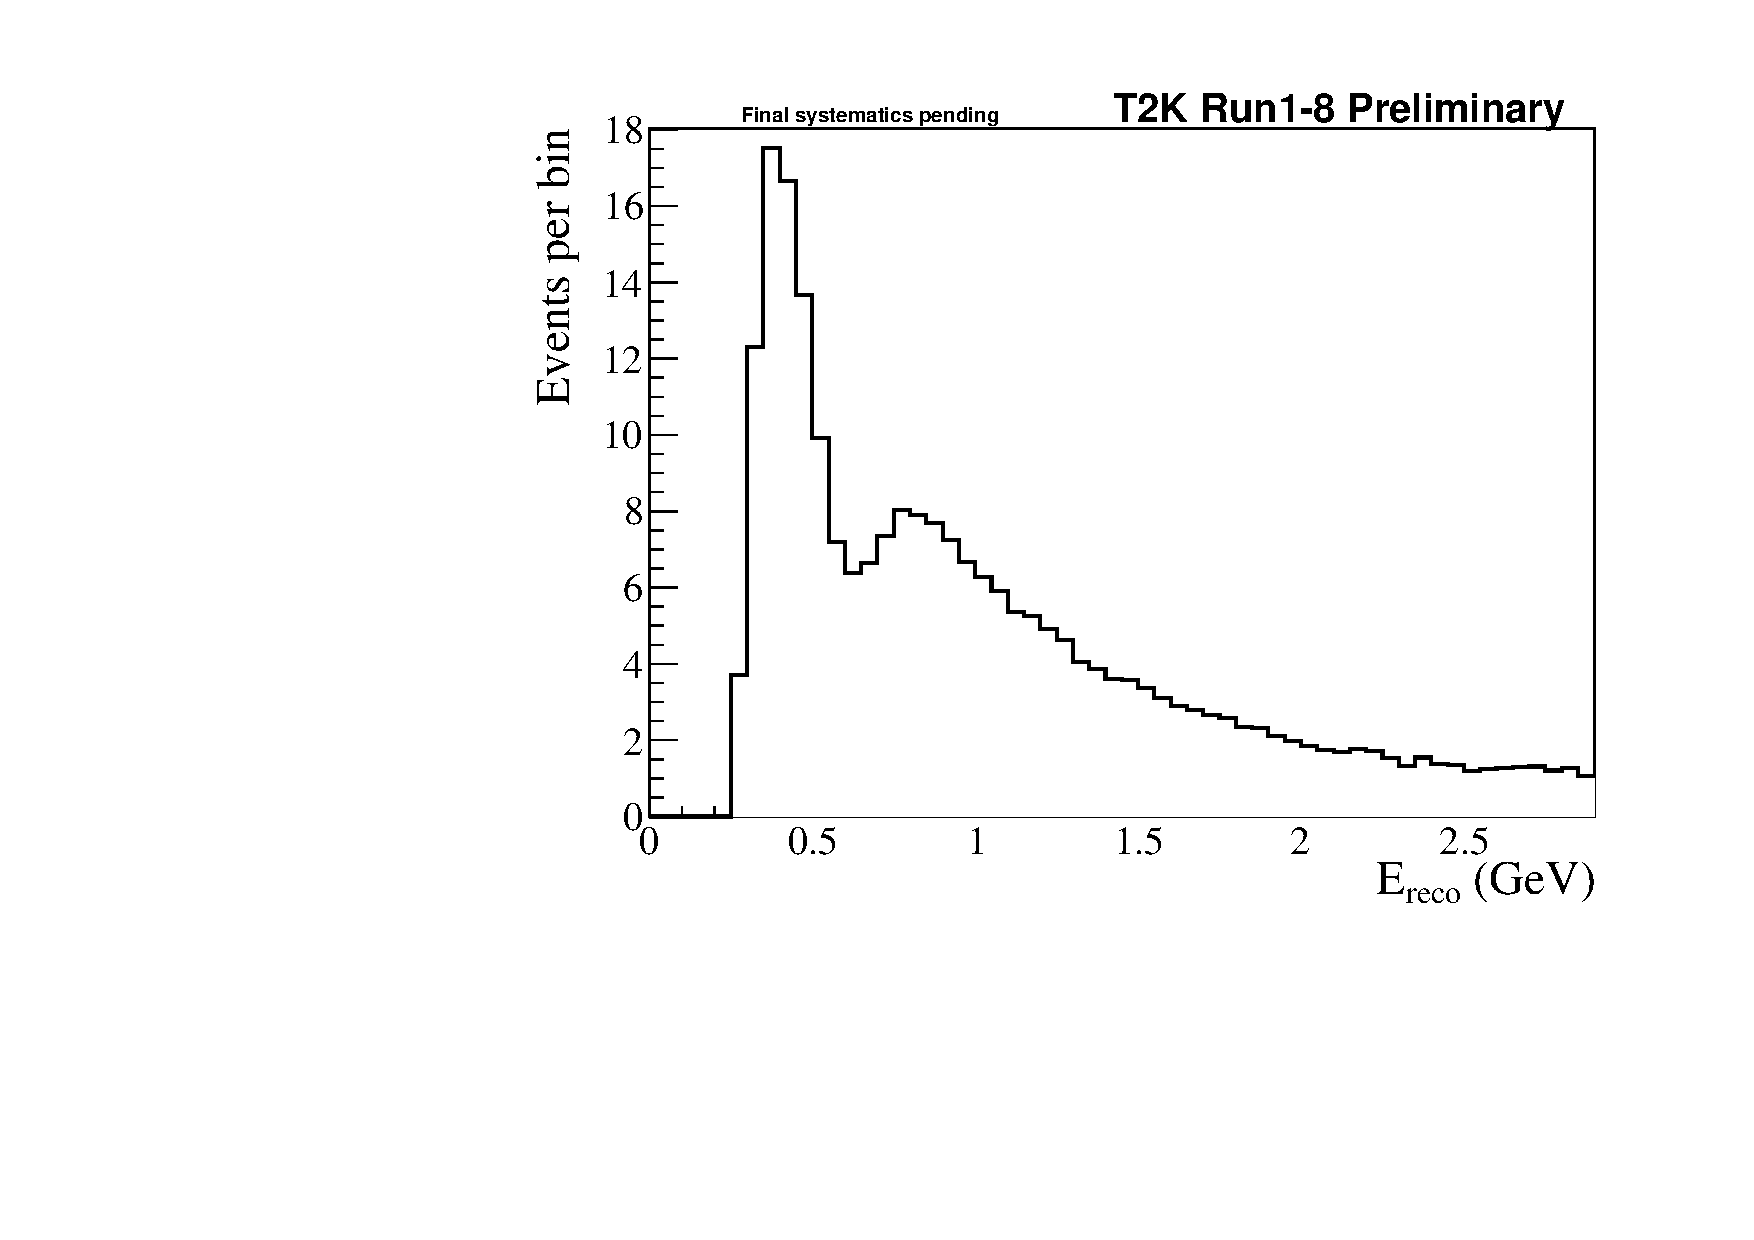
\includegraphics[width=0.9\textwidth]{systematics/envelopes/sk_errors/sk_error_table_1Rmu_osc_envelope}
		\caption{Muon-like, neutrino mode}
	\end{subfigure}
	\begin{subfigure}[b]{0.49\textwidth}
		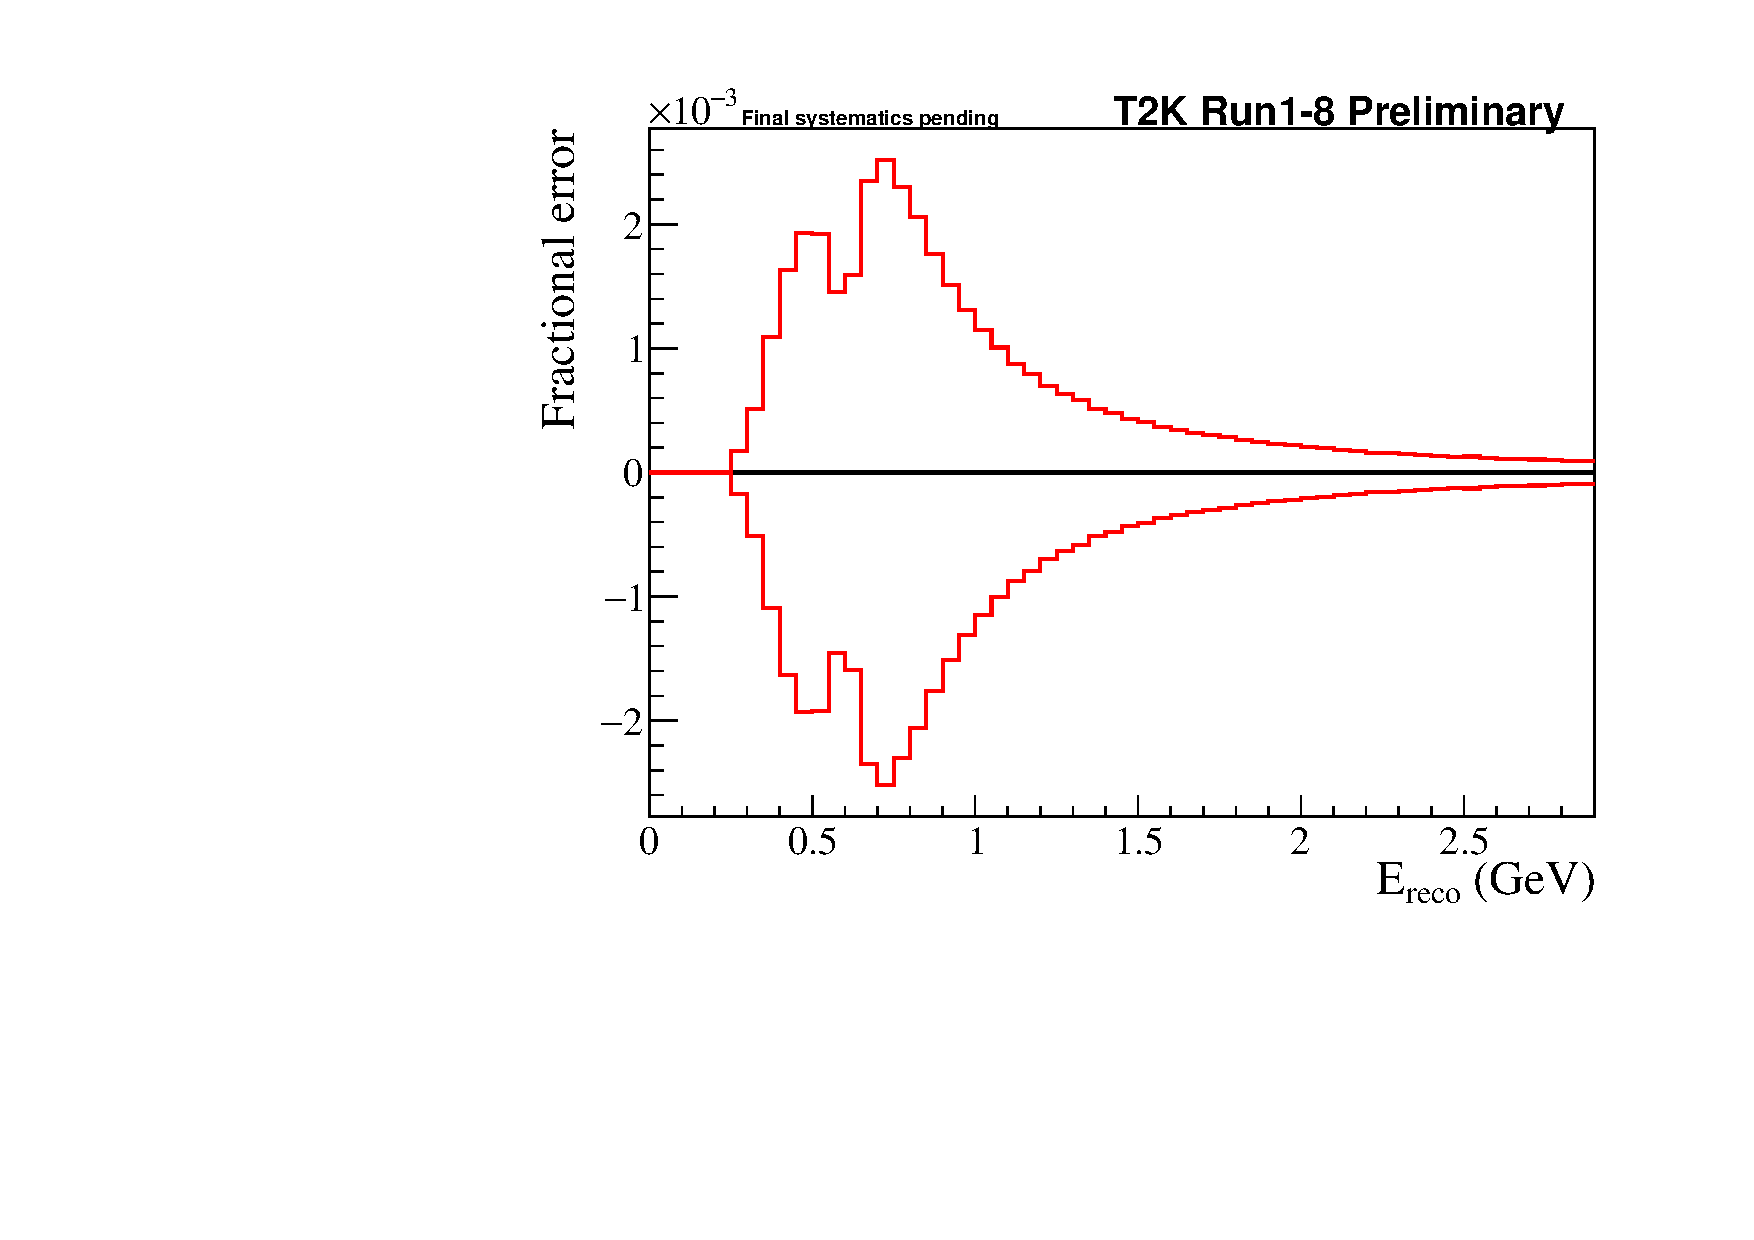
\includegraphics[width=0.9\textwidth]{systematics/envelopes/sk_errors/sk_error_table_1Rmu_osc_envelope_fractional}
		\caption{Muon-like, neutrino mode}
	\end{subfigure}
	\begin{subfigure}[b]{0.49\textwidth}
		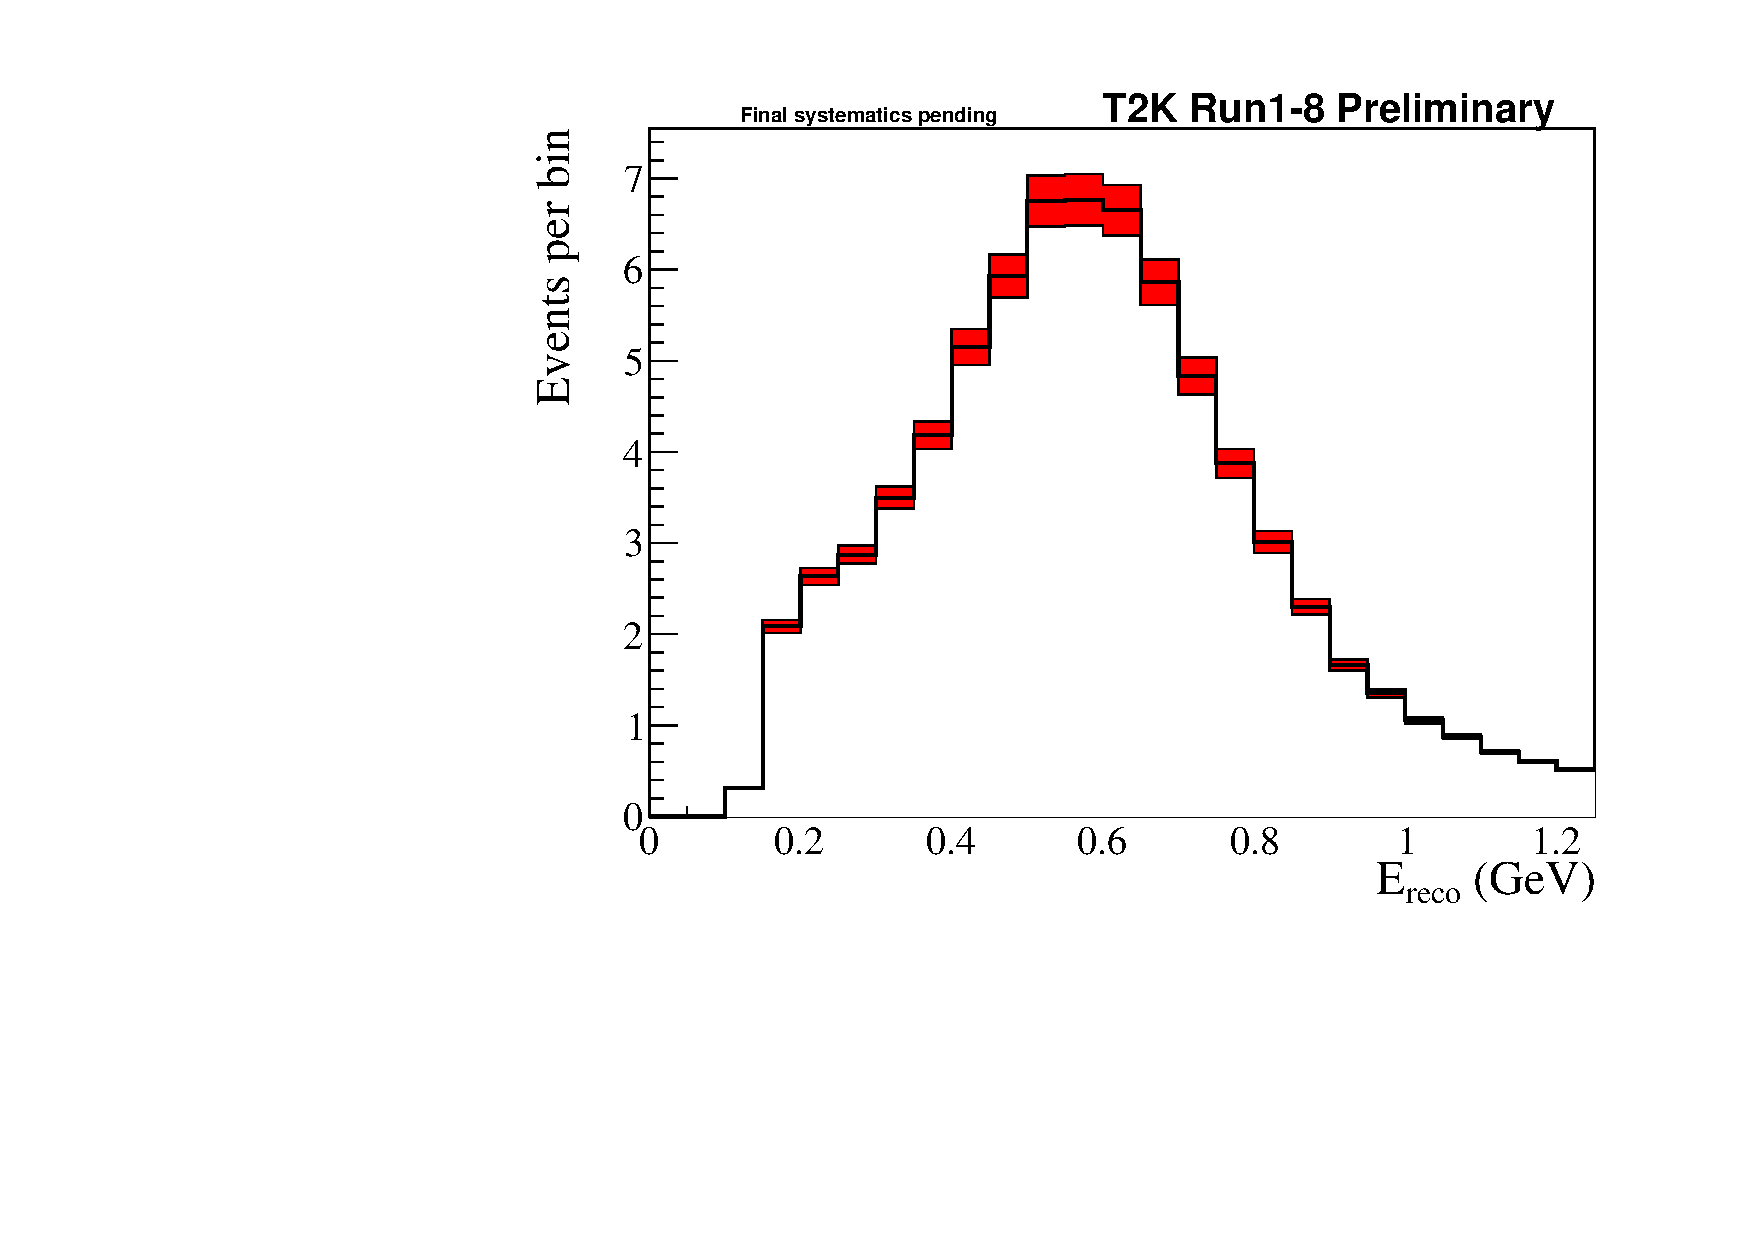
\includegraphics[width=0.9\textwidth]{systematics/envelopes/sk_errors/sk_error_table_1Re_osc_envelope}
		\caption{Electron-like, neutrino mode}
	\end{subfigure}
	\begin{subfigure}[b]{0.49\textwidth}
		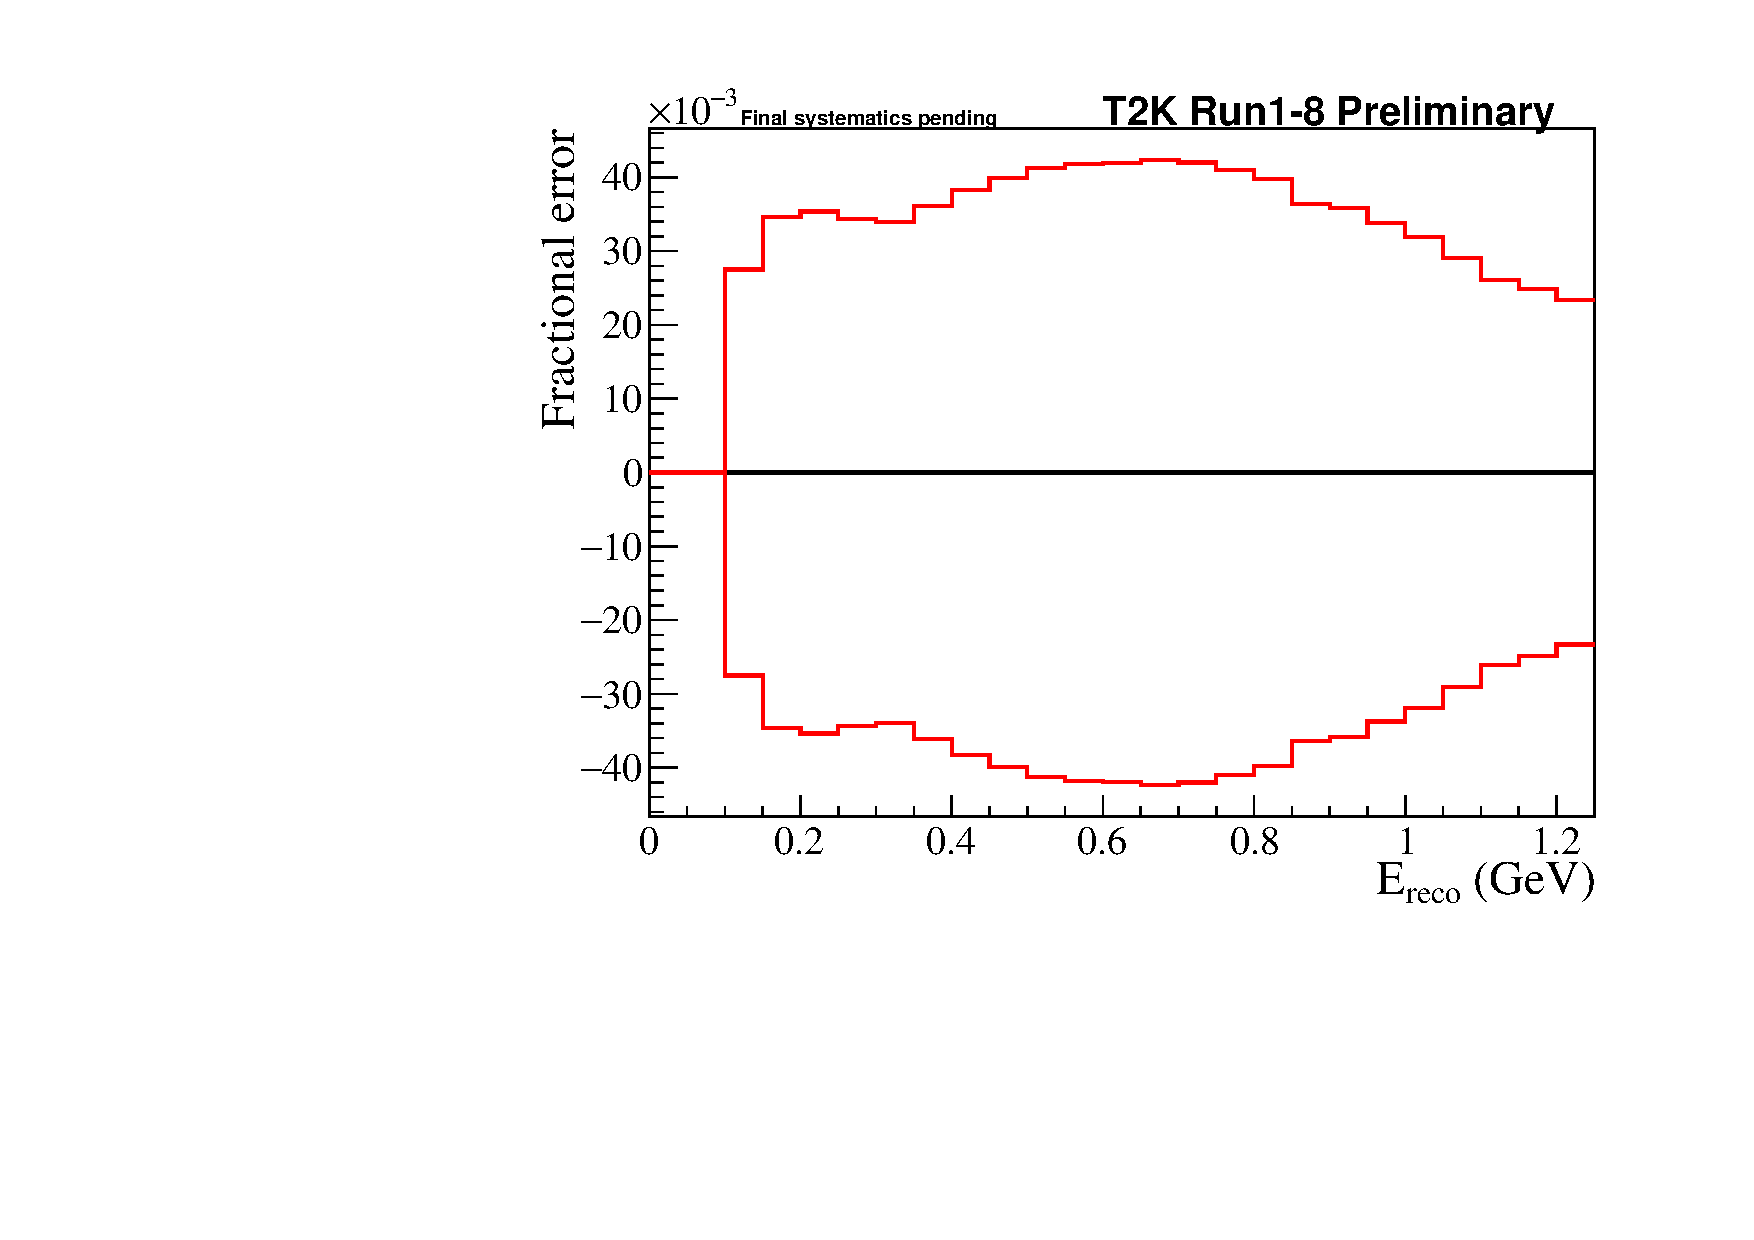
\includegraphics[width=0.9\textwidth]{systematics/envelopes/sk_errors/sk_error_table_1Re_osc_envelope_fractional}
		\caption{Electron-like, neutrino mode}
	\end{subfigure}
	\begin{subfigure}[b]{0.49\textwidth}
		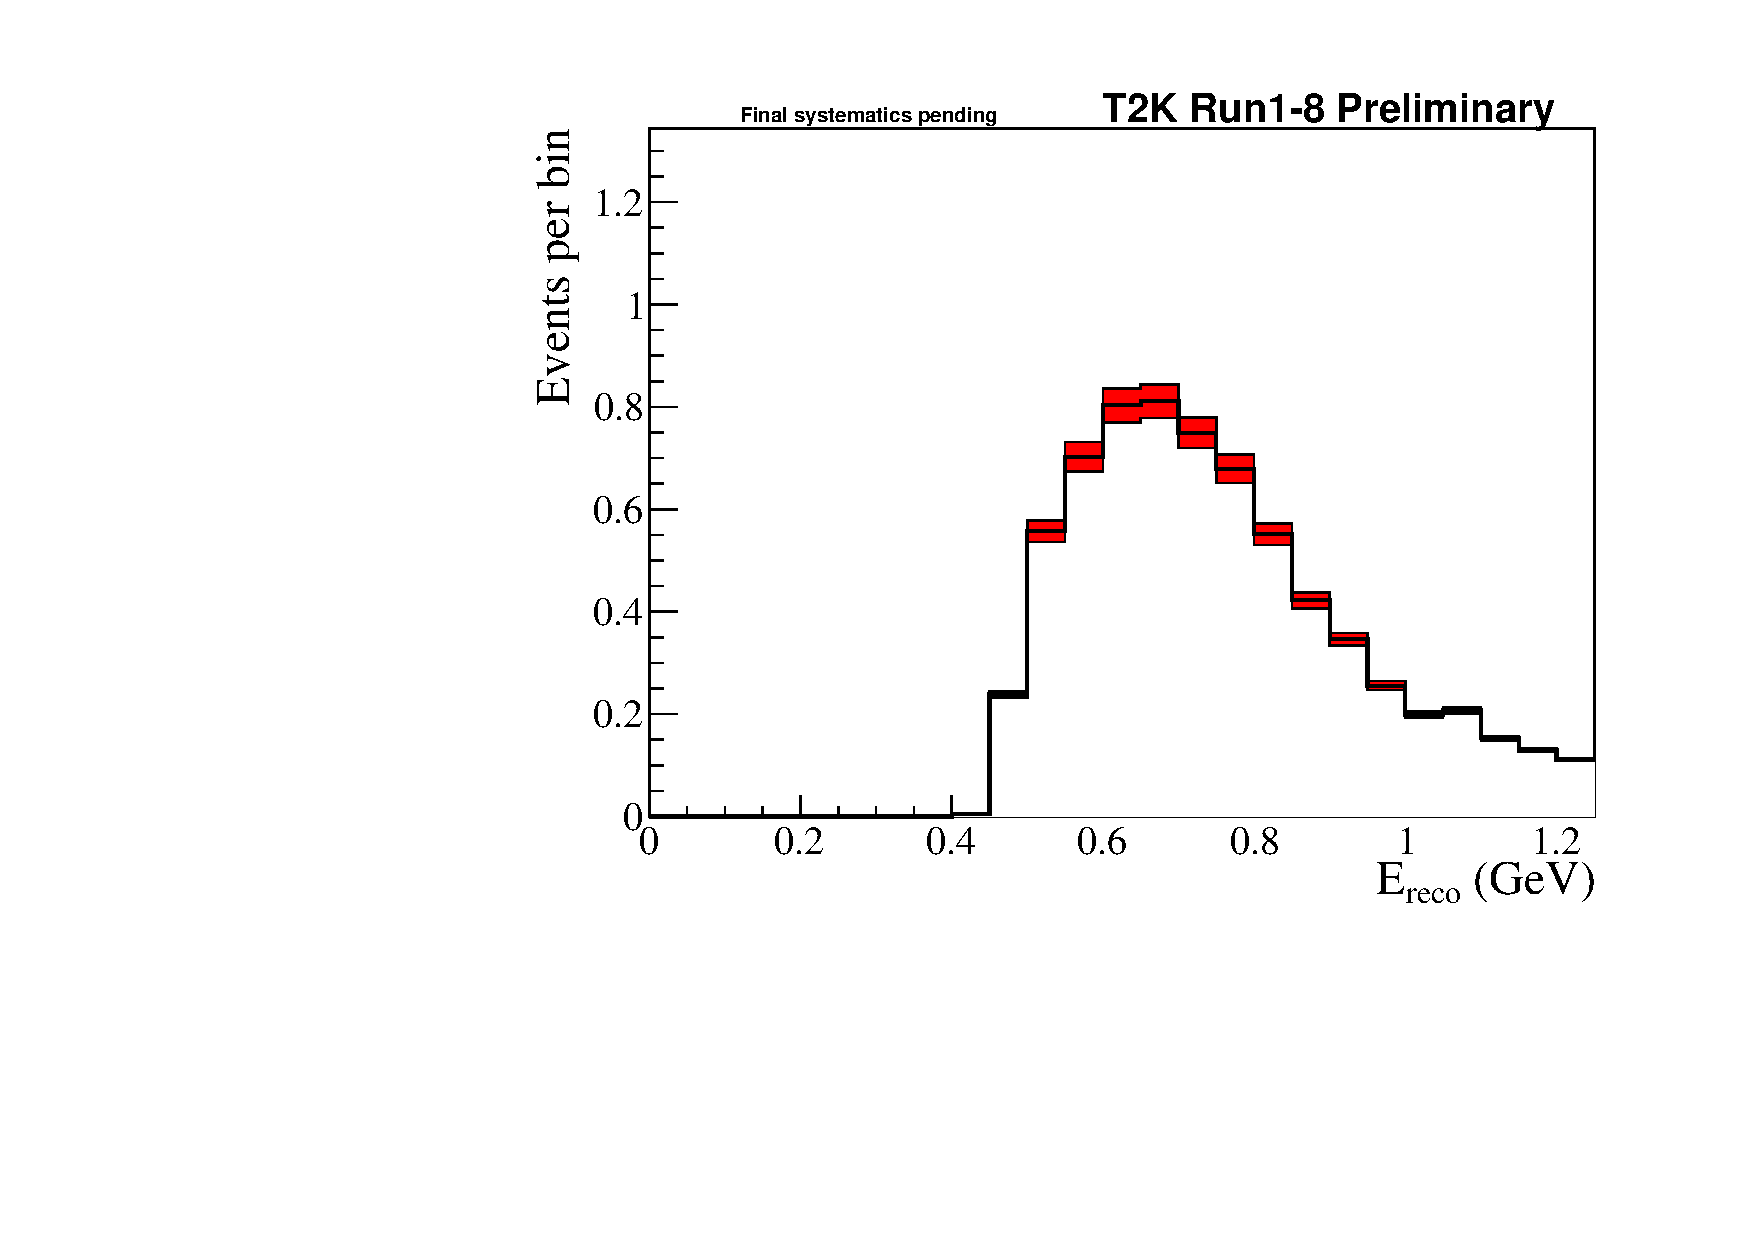
\includegraphics[width=0.9\textwidth]{systematics/envelopes/sk_errors/sk_error_table_MultiRe_osc_envelope}
		\caption{\nueCConepi-like, neutrino mode}
	\end{subfigure}
	\begin{subfigure}[b]{0.49\textwidth}
		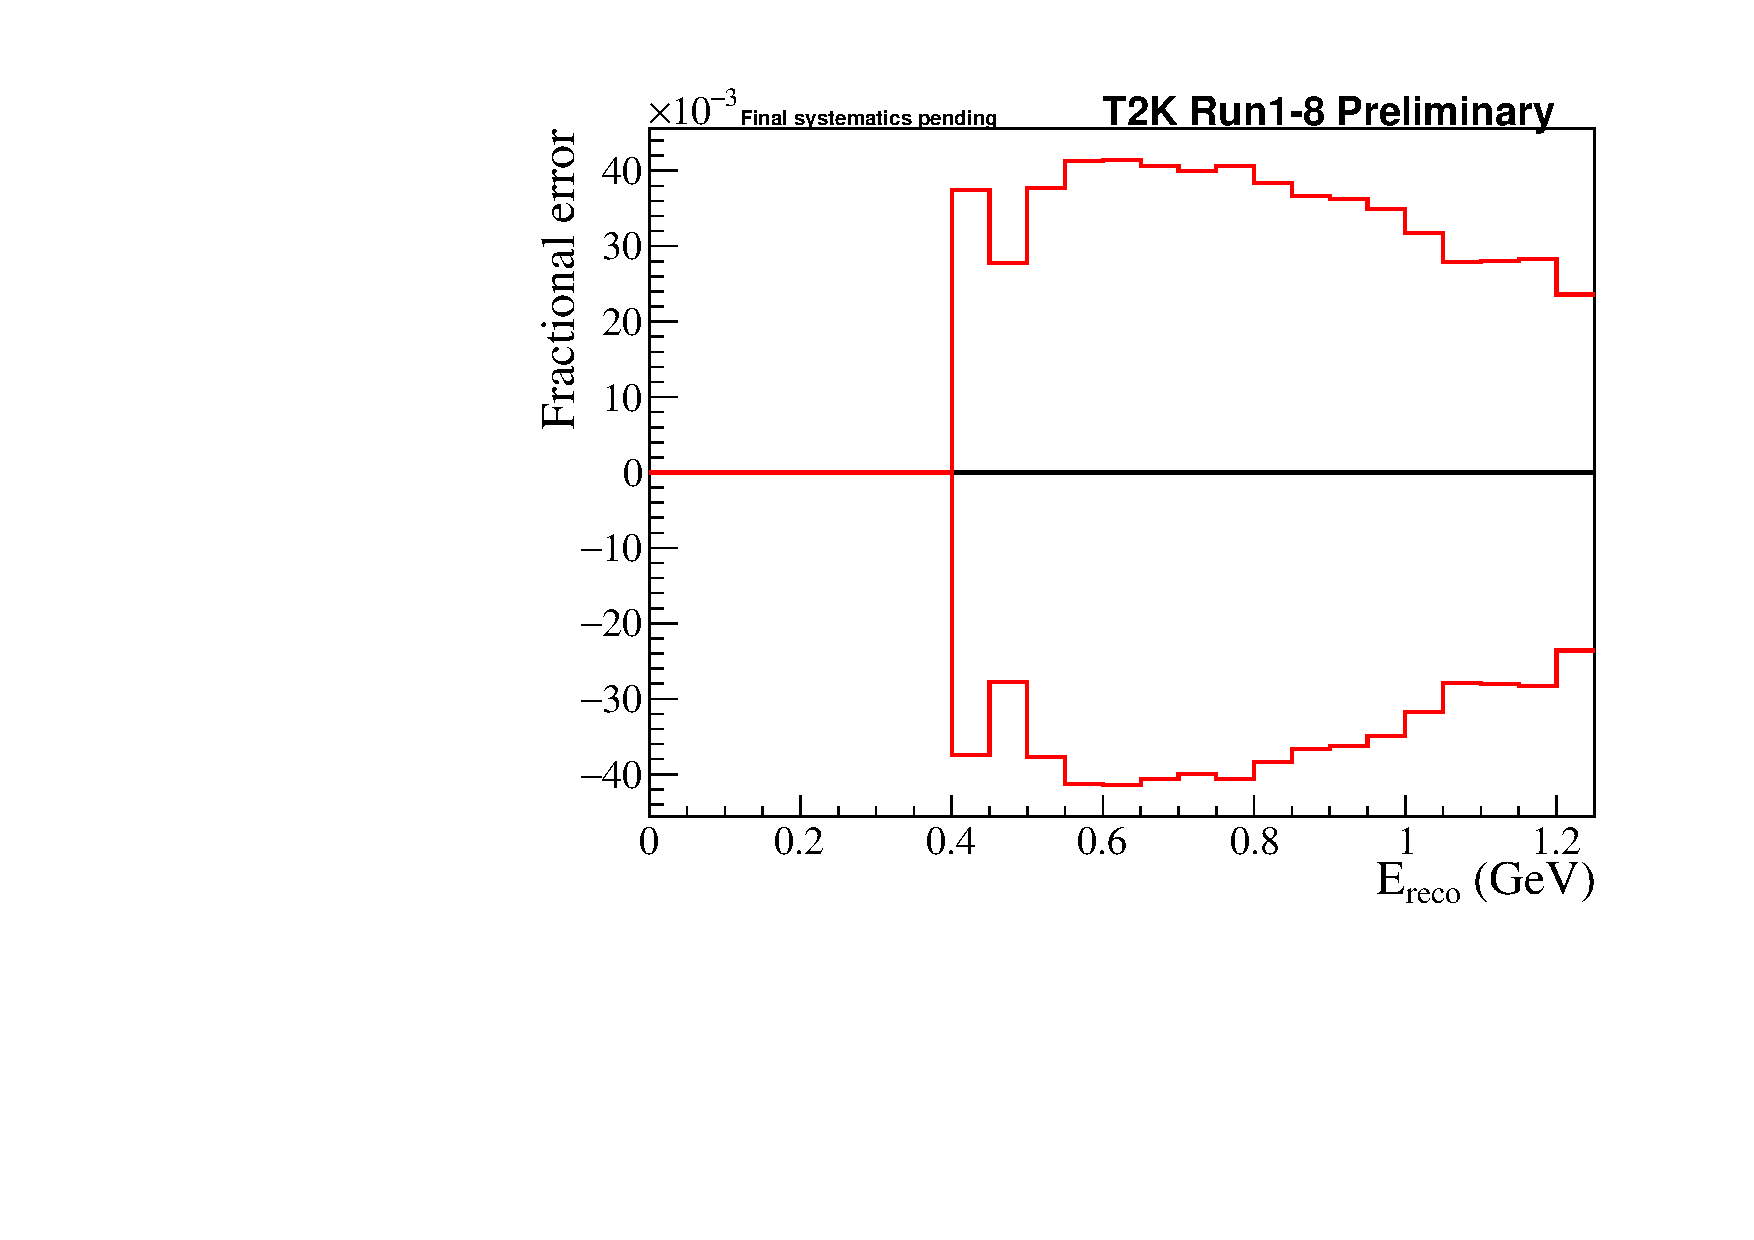
\includegraphics[width=0.9\textwidth]{systematics/envelopes/sk_errors/sk_error_table_MultiRe_osc_envelope_fractional}
		\caption{\nueCConepi-like, neutrino mode}
	\end{subfigure}
	\caption {
		Error envelopes (left) and fractional errors (right) for the reconstructed neutrino energy spectrum for all oscillation nuisance parameters. \num{1e4} toys are generated for the Asimov data set A with randomized systematic parameters with correlations taken into account. Since \deltacp, \ssqthtwothree, \dmsqtwothree and the mass hierarchy will be measured, only the uncertainty on \ssqthonethree, \ssqthonetwo and \dmsqonetwo are taken into account.
	}
	\label{fig:sk_envelopes_osc}
\end{figure*}
\clearpage

\begin{figure*}
	\center
	\begin{subfigure}[b]{0.49\textwidth}
		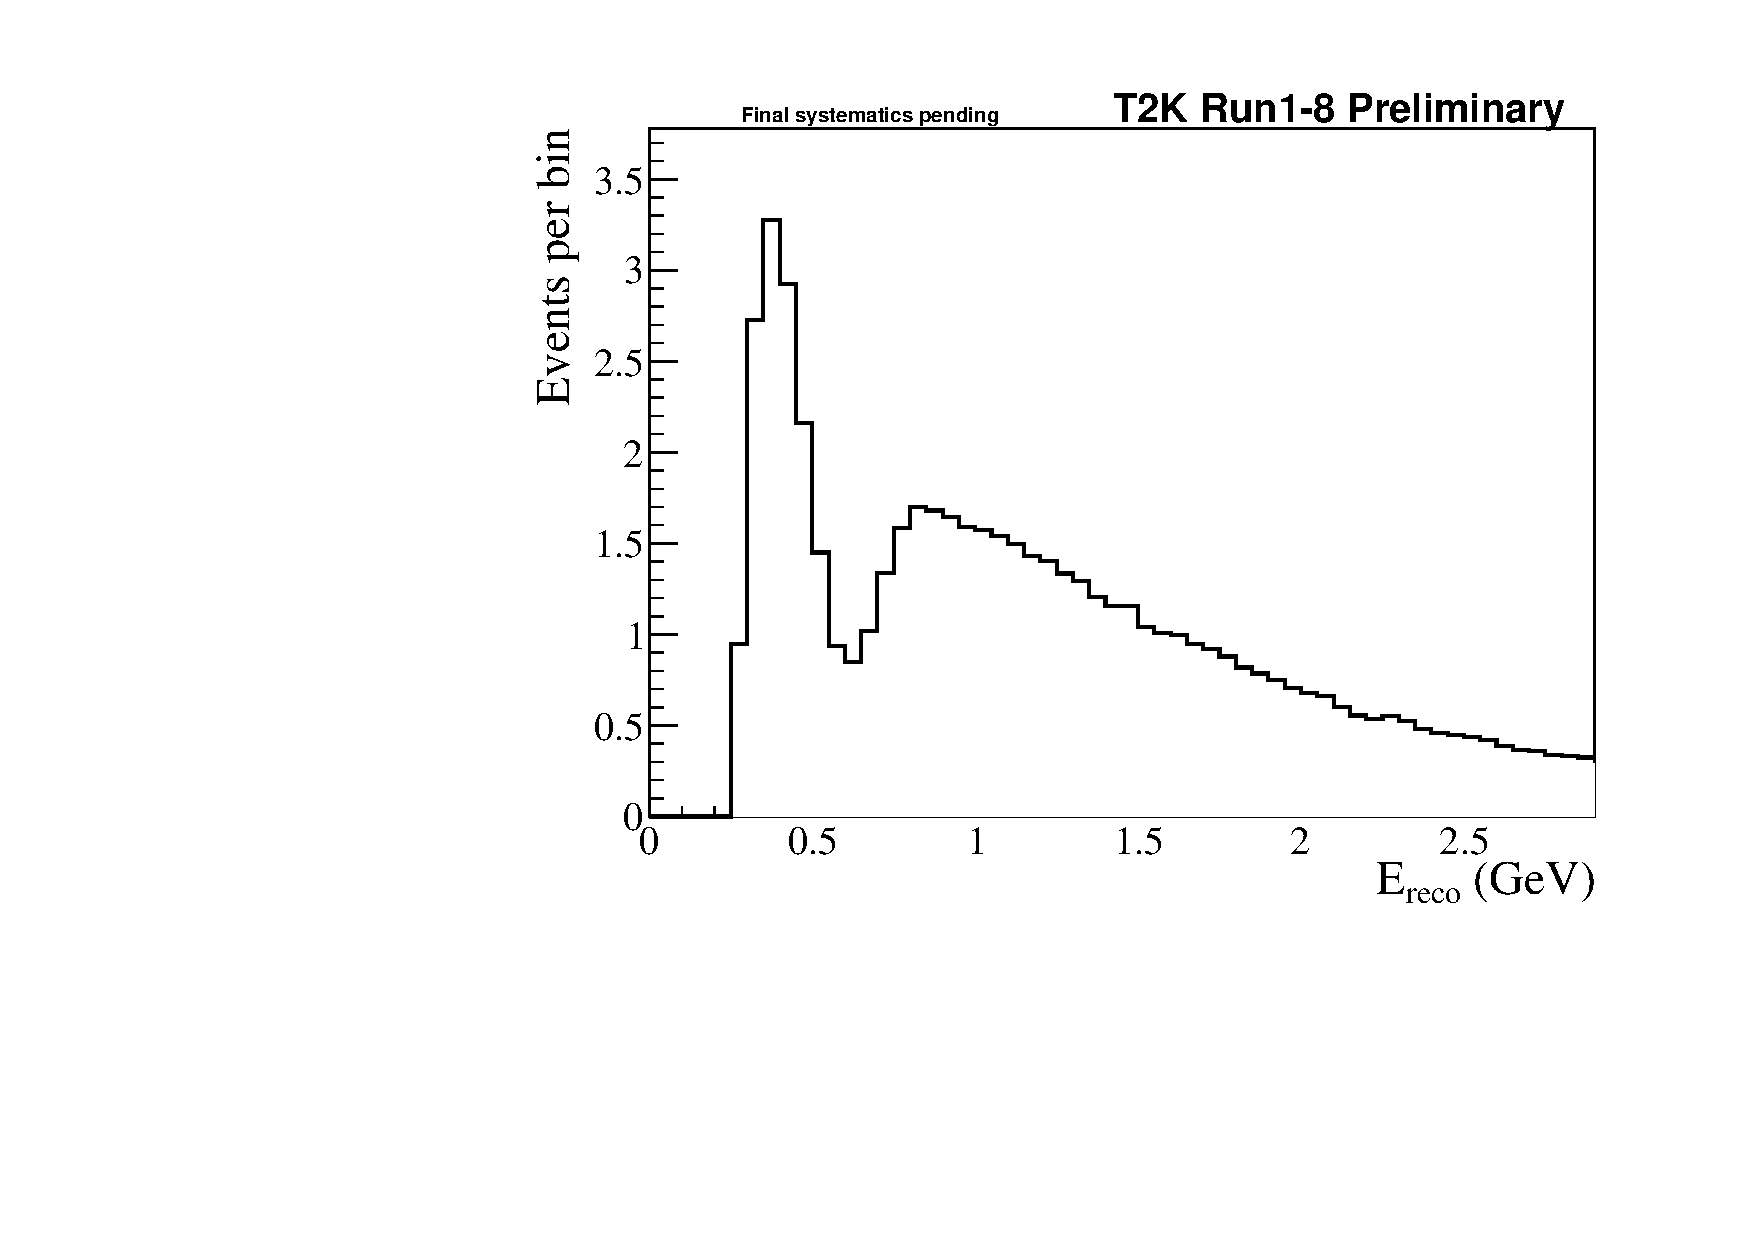
\includegraphics[width=0.9\textwidth]{systematics/envelopes/sk_errors/sk_error_table_RHC1Rmu_osc_envelope}
		\caption{Muon-like, antineutrino mode}
	\end{subfigure}
	\begin{subfigure}[b]{0.49\textwidth}
		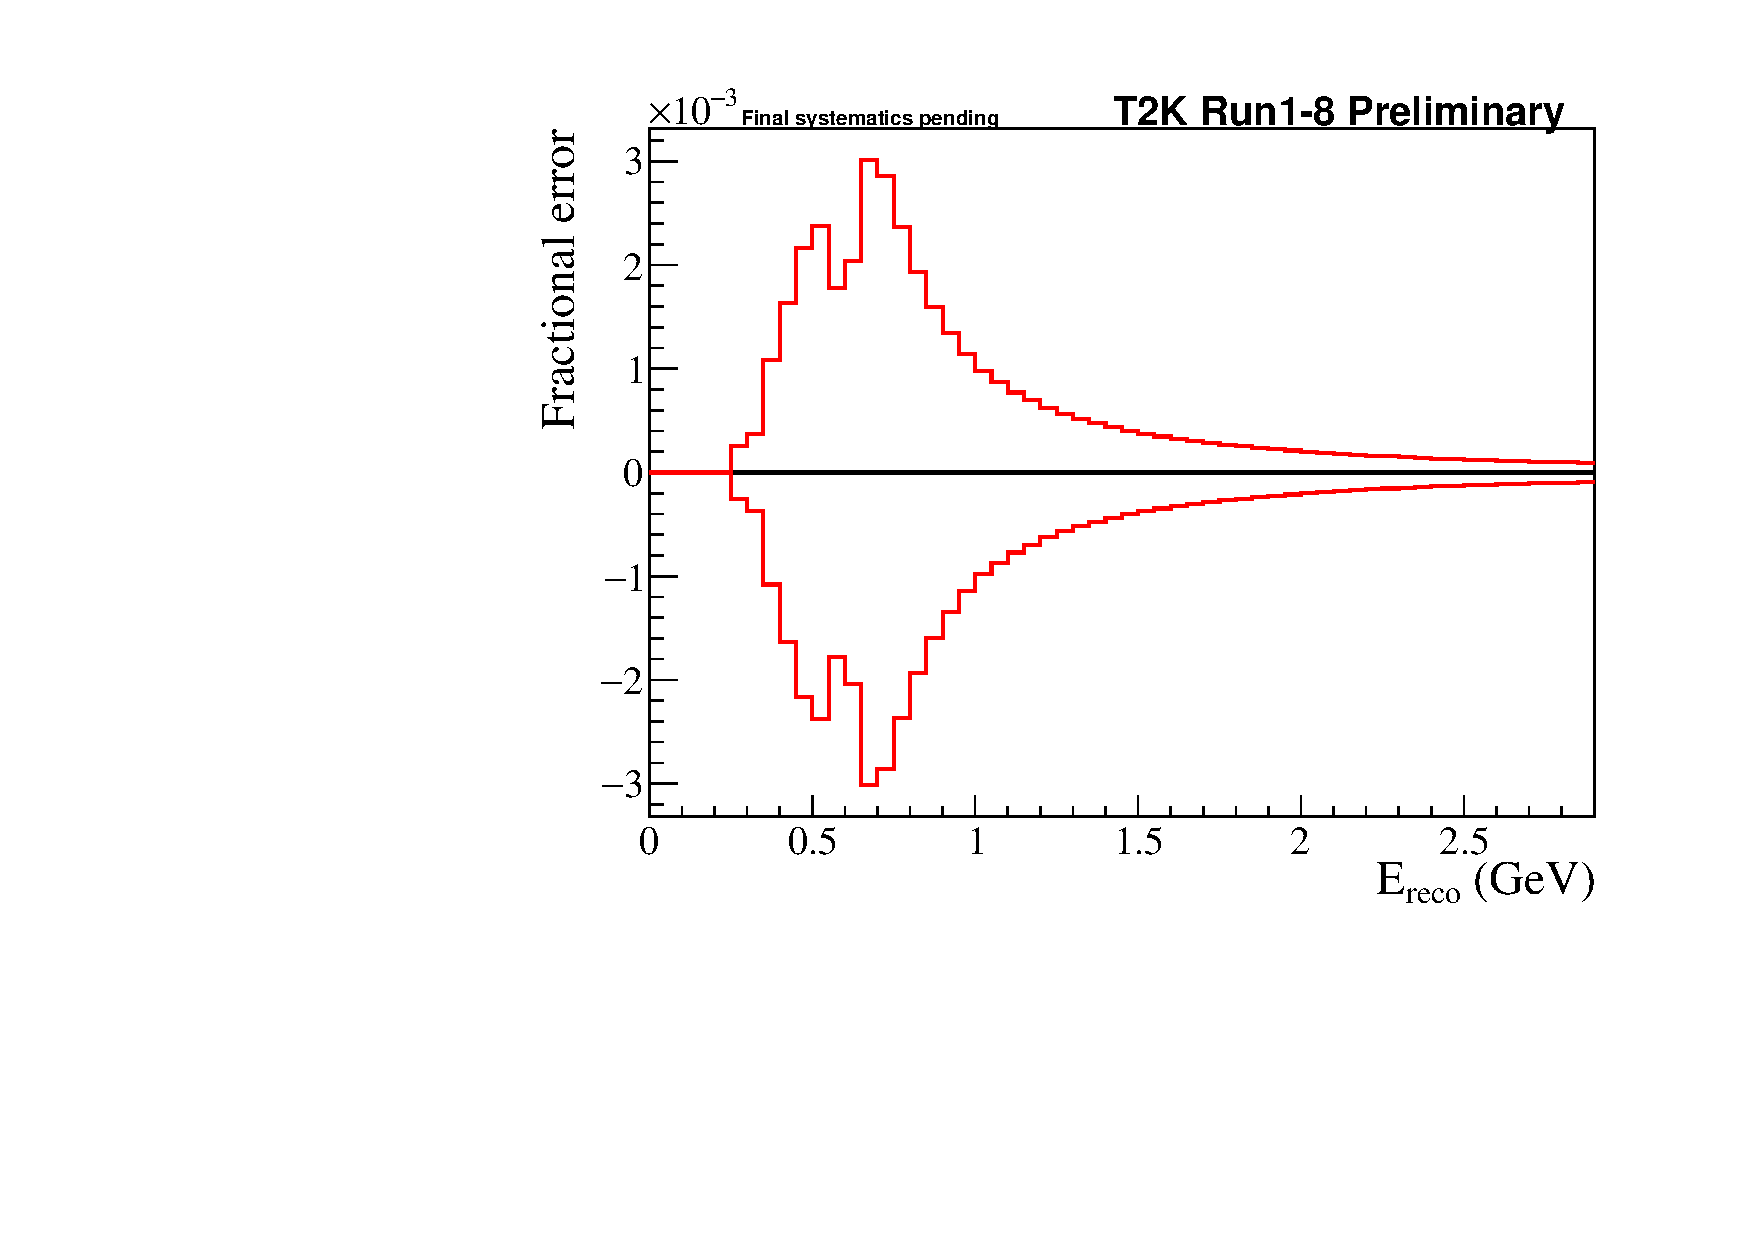
\includegraphics[width=0.9\textwidth]{systematics/envelopes/sk_errors/sk_error_table_RHC1Rmu_osc_envelope_fractional}
		\caption{Muon-like, antineutrino mode}
	\end{subfigure}
	\begin{subfigure}[b]{0.49\textwidth}
		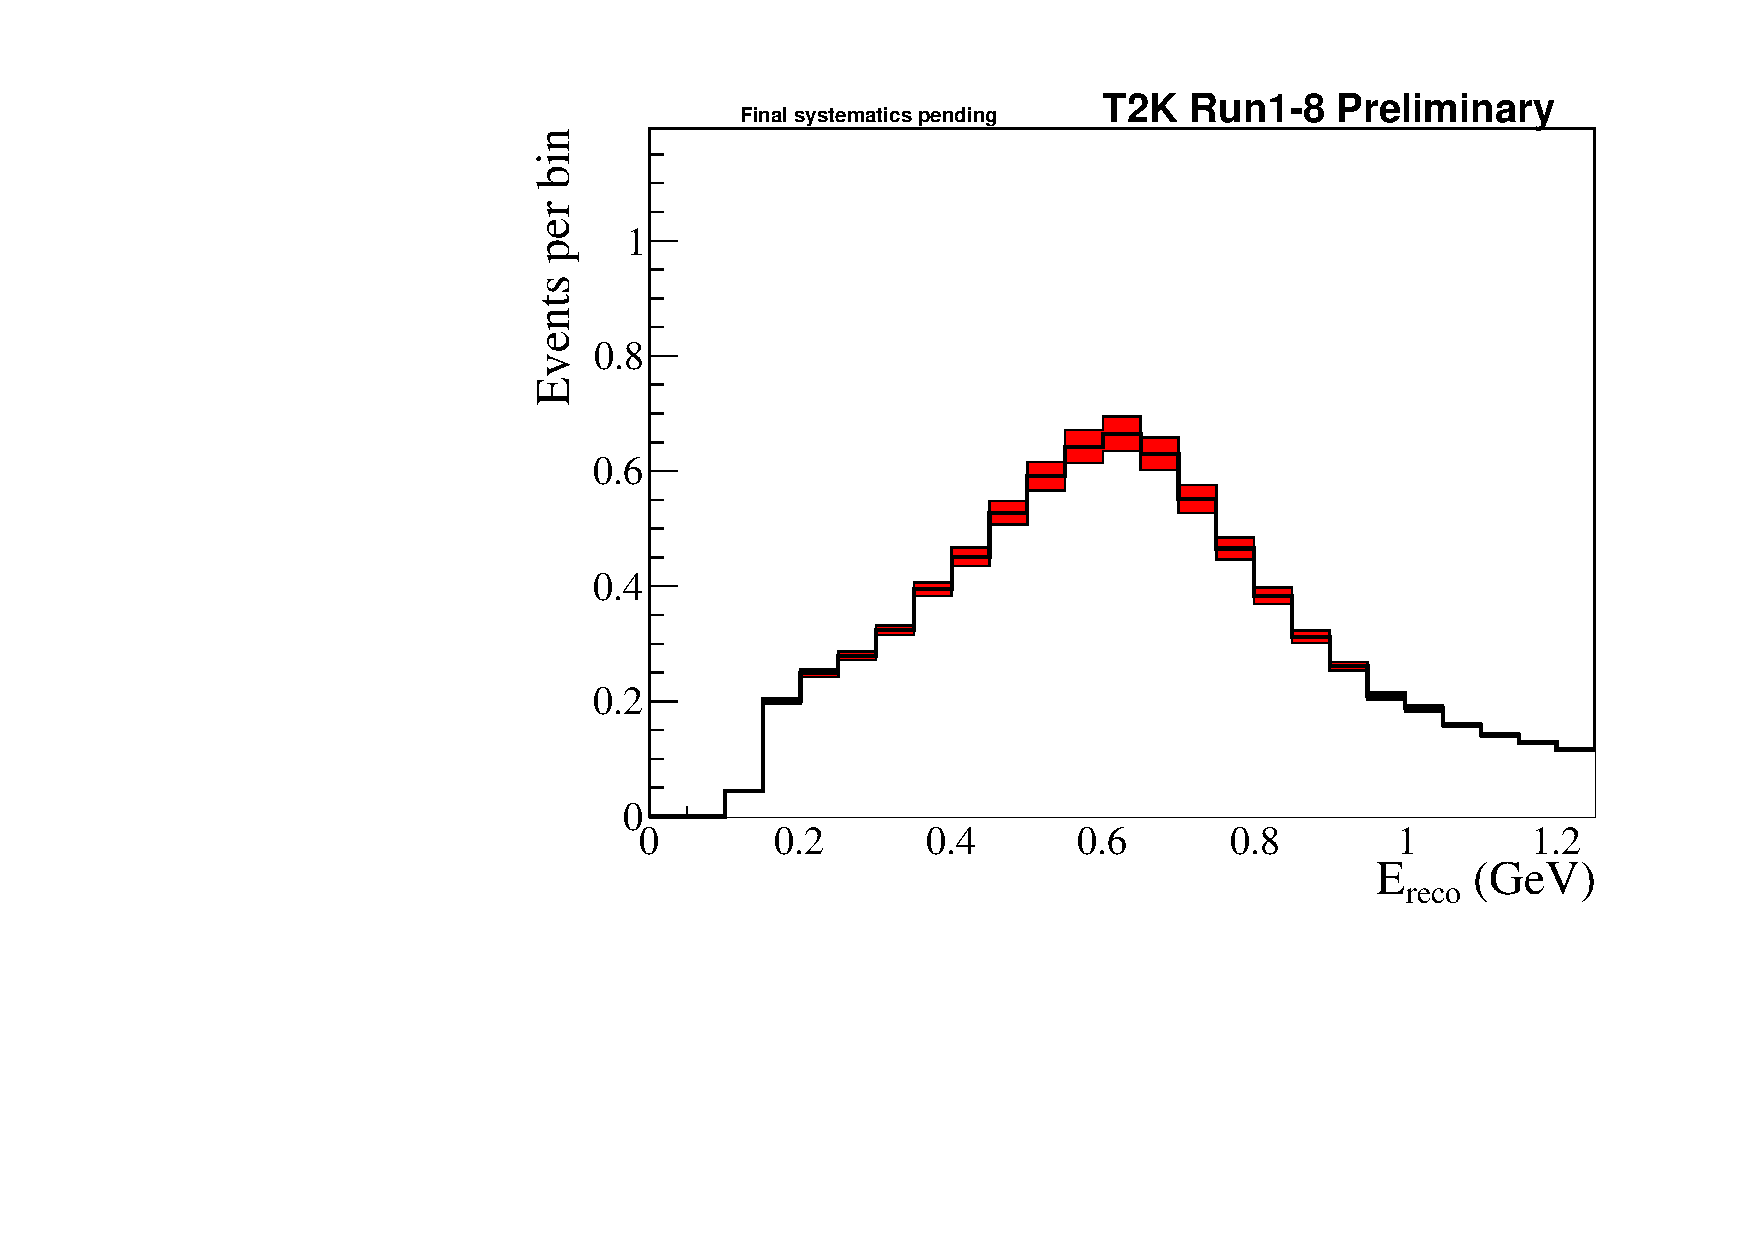
\includegraphics[width=0.9\textwidth]{systematics/envelopes/sk_errors/sk_error_table_RHC1Re_osc_envelope}
		\caption{Electron-like antineutrino mode}
	\end{subfigure}
	\begin{subfigure}[b]{0.49\textwidth}
		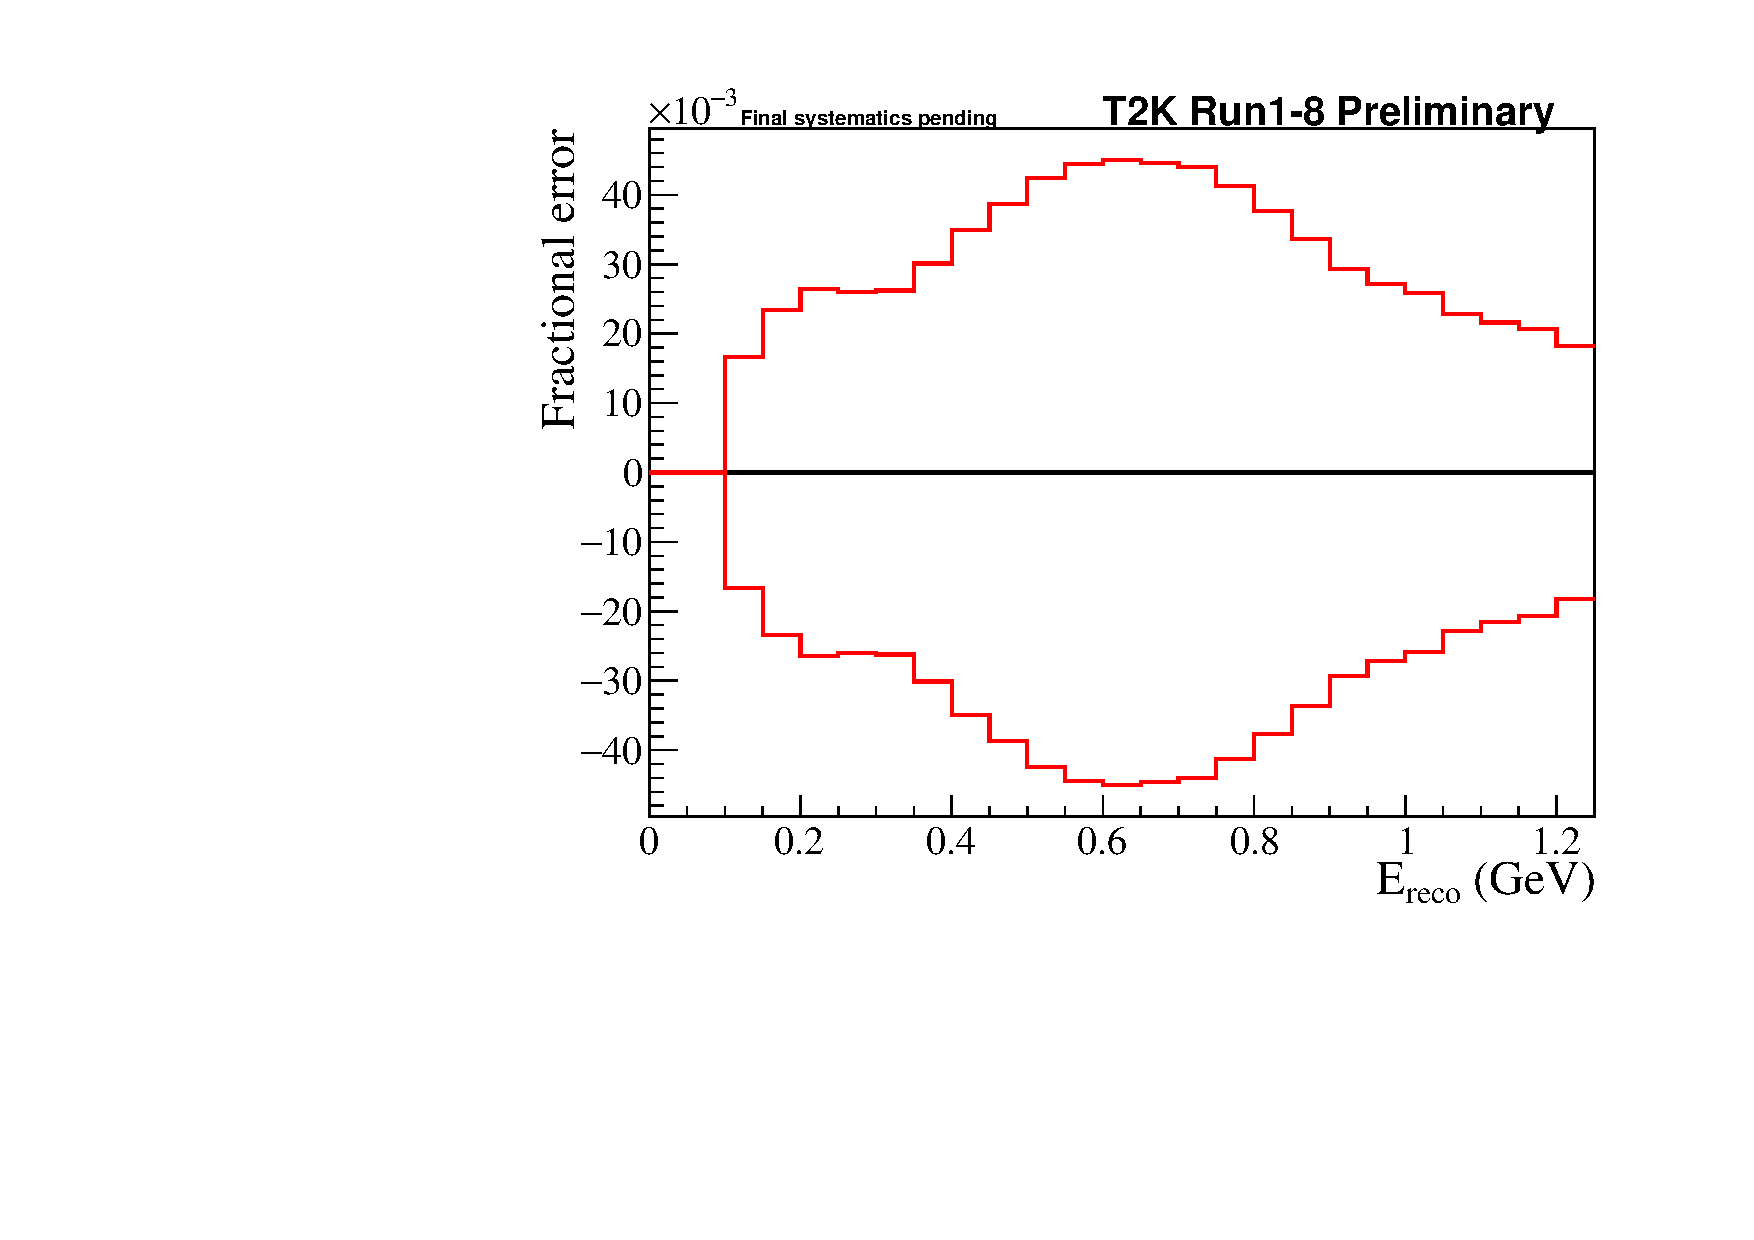
\includegraphics[width=0.9\textwidth]{systematics/envelopes/sk_errors/sk_error_table_RHC1Re_osc_envelope_fractional}
		\caption{Electron-like antineutrino mode}
	\end{subfigure}
	\caption {
		Error envelopes (left) and fractional errors (right) for the reconstructed neutrino energy spectrum for all oscillation nuisance parameters. \num{1e4} toys are generated for the Asimov data set A with randomized systematic parameters with correlations taken into account. Since \deltacp, \ssqthtwothree, \dmsqtwothree and the mass hierarchy will be measured, only the uncertainty on \ssqthonethree, \ssqthonetwo and \dmsqonetwo are taken into account.
	}
	\label{fig:sk_envelopes_osc_b}
\end{figure*}
\clearpage